% !TEX root = main.tex

\chapter{Background}
\label{ch:background}
\noindent


\section{WebAssembly}

% breif overview
WebAssembly is a low-level bytecode language that is safe, fast, portable, and
compact~\cite{wasm}.
It is widely used as a compile target for web applications.
Not only that, other areas such as edge computing~\cite{wasm-edge},
IoT~\cite{wasm-iot}, and block chains~\cite{wasm-block} deploy the advantages
of WebAssembly.

% risk of implementation divergence
There are dozens of WebAssembly engines; all the browsers have there own
implementations of WebAssembly with multiple tiers, and there are many engines
that target for specific areas including embedded systems and edge computing.
However, as WebAssembly should be portable across these implementations, it risks
the implementations divergence.

% rigorous standardization -> spec is rigorous: formal notation & prose notation
To mitigate this problem, WebAssembly has been standardized very rigourously by
the W3C~\cite{wasm-w3c}.
Especially, WebAssembly specification is written very rigorously.
It describes the semantics of WebAssembly in two forms: formal notation and
prose notation.
Formal notation uses mathematical rules to compactly describe the semantics,
and it is used for proofs such as type soundness.
On the other hand, prose notation uses psudocodes to explain the semantics step
by step.
Most WebAssembly users and engine developers are not familiar with
mathematical rules, so they utilize the prose notation.

% structure
A WebAssembly program is comprised of \textit{modules}.
A module is the unit of deployment, loading, and compilation, which consists of
definitions such as functions, globals, and memories.
A module is instantiated to validate the module, allocate each definition to
the data structure named \textit{store}.
This results in module instance, a runtime representation for the module.
After the instantiation, functions can be invoked for the execution.

\begin{figure}[t]
    \centerline{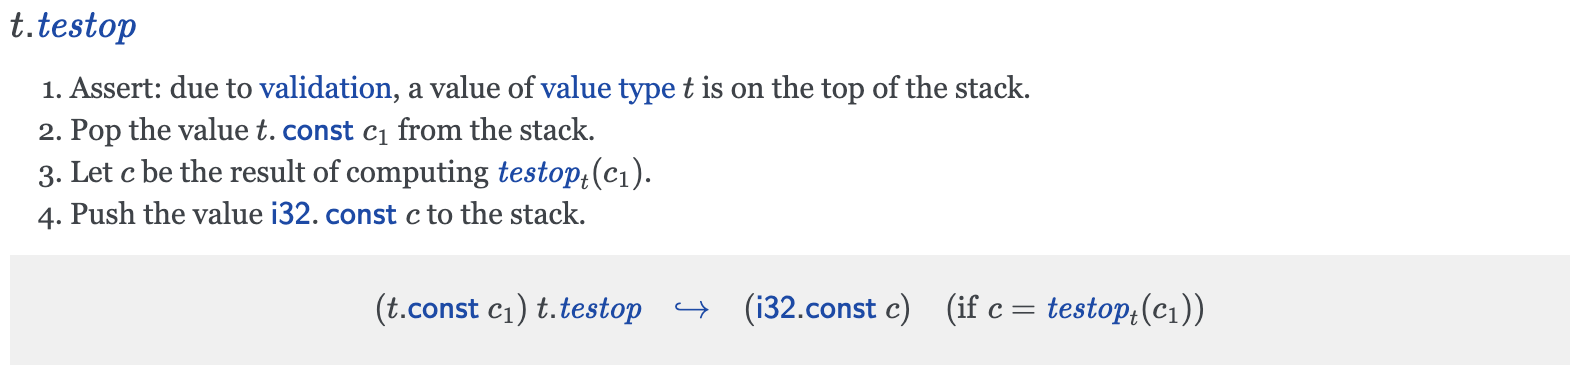
\includegraphics[width=15cm]{fig/testop}}
    \caption[Enter the caption title here]{\texttt{testop} instruction} \label{fig:testop}
\end{figure}

% execution
WebAssembly execution is based on a stack machine.
An instruction consumes values in the stack as operands, produces the
resulting values, and pushes them to the stack.
\cref{fig:testop} is the WebAssembly specification for the \texttt{testop}
instruction.
Prose notation is written in the upper part, and formal notation is written in
the lower grey box.
In the prose notation, it pops a value from the stack, performs a test
operation, and pushes the result to the stack.
It is written compactly in the form of reduction rule in the formal notation
which consists of LHS, RHS, and premises: $(t.const ~ c_1) ~ t.testop$,
$(i32.const ~ c)$, and $c = testop_t(c_1)$.
The LHS means that the value at the top of the stack is $(t.const ~ c_1)$,
and an instruction to execute is $t.testop$.
The RHS means that the value at the top of the stack is changed to $(i32.const
~ c)$, and this happens when the premise $c = testop_t(c_1)$ is satisfied.

% control structure
The stack stores not only the input and output values of the instructions but also
structures related to the control flow.
A \textit{call frame} and a \textit{label} are used for function call and
branching, respectively.
In exception handling proposal, there is a \textit{handler} for exception
handling, and other strucutres could be introduced in the future.
How these control structures are used for the control flow will be discussed in
\cref{sec:control flow in official prose}. \\
\red{TODO: remove dangling section header}

\section{SpecTec}
